\documentclass{article}
\usepackage{polyglossia}
\usepackage{graphicx}
\setdefaultlanguage{slovak}
\begin{document}
\hrule
\medskip
\begin{center}
\textbf{\huge RIEŠENIE}
\end{center}
\medskip
\hrule
\medskip
\large
Vypočítame dĺžku Jožkových nôh $N$.
Vieme, že $N = \frac{4}{7} \times J_v = \frac{4}{7} \times 2 = \frac{8}{7} \approx 1.142857 m  $.\\
Teraz si zistime dĺžku jeho kroku $J_k$.
Nakreslíme si obrázok:
\medskip
\begin{center}
	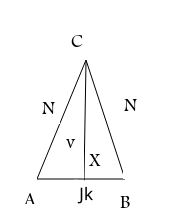
\includegraphics{imagex/trojuholnik.png}
\end{center}

\noindent Teraz si zistíme výšku $v$. Zo zadania vidíme že keď stojí Jožko rozkročený, je o $\frac{1}{40}$ svojej výšky nižší.\\
Jeho výška je 2m, z čoho $\frac{1}{40}$ je $0.05m = 5cm$.
$v$ by teda malo byť $N - 0.05 = 1.092857$.
Na obrázku vidíme pravouhlý trojuholník $XBC$
\medskip
\hrule
\end{document}
